\documentclass[a4paper]{book}
\usepackage{a4wide}
\usepackage{makeidx}
\usepackage{graphicx}
\usepackage{multicol}
\usepackage{float}
\usepackage{listings}
\usepackage{color}
\usepackage{textcomp}
\usepackage{alltt}
\usepackage{times}
\usepackage{ifpdf}
\ifpdf
\usepackage[pdftex,
            pagebackref=true,
            colorlinks=true,
            linkcolor=blue,
            unicode
           ]{hyperref}
\else
\usepackage[ps2pdf,
            pagebackref=true,
            colorlinks=true,
            linkcolor=blue,
            unicode
           ]{hyperref}
\usepackage{pspicture}
\fi
\usepackage[utf8]{inputenc}
\usepackage{doxygen}
\lstset{language=C++,inputencoding=utf8,basicstyle=\footnotesize,breaklines=true,breakatwhitespace=true,tabsize=8,numbers=left }
\makeindex
\setcounter{tocdepth}{3}
\renewcommand{\footrulewidth}{0.4pt}
\begin{document}
\hypersetup{pageanchor=false}
\begin{titlepage}
\vspace*{7cm}
\begin{center}
{\Large Reference Manual}\\
\vspace*{1cm}
{\large Generated by Doxygen 1.6.1}\\
\vspace*{0.5cm}
{\small Sun Nov 8 23:56:52 2015}\\
\end{center}
\end{titlepage}
\clearemptydoublepage
\pagenumbering{roman}
\tableofcontents
\clearemptydoublepage
\pagenumbering{arabic}
\hypersetup{pageanchor=true}
\chapter{Class Index}
\section{Class Hierarchy}
This inheritance list is sorted roughly, but not completely, alphabetically:\begin{DoxyCompactList}
\item \contentsline{section}{Character}{\pageref{classCharacter}}{}
\begin{DoxyCompactList}
\item \contentsline{section}{Enemy}{\pageref{classEnemy}}{}
\item \contentsline{section}{Player}{\pageref{classPlayer}}{}
\end{DoxyCompactList}
\item \contentsline{section}{Enviros}{\pageref{classEnviros}}{}
\begin{DoxyCompactList}
\item \contentsline{section}{Castle}{\pageref{classCastle}}{}
\item \contentsline{section}{Cave}{\pageref{classCave}}{}
\item \contentsline{section}{Forest}{\pageref{classForest}}{}
\item \contentsline{section}{Village}{\pageref{classVillage}}{}
\end{DoxyCompactList}
\item \contentsline{section}{invalid\_\-input}{\pageref{classinvalid__input}}{}
\item \contentsline{section}{invalid\_\-move\_\-error}{\pageref{classinvalid__move__error}}{}
\item \contentsline{section}{Items}{\pageref{classItems}}{}
\begin{DoxyCompactList}
\item \contentsline{section}{Bomb}{\pageref{classBomb}}{}
\item \contentsline{section}{Potion}{\pageref{classPotion}}{}
\item \contentsline{section}{SuperPotion}{\pageref{classSuperPotion}}{}
\end{DoxyCompactList}
\item \contentsline{section}{LandofTorvold}{\pageref{classLandofTorvold}}{}
\item \contentsline{section}{Questions}{\pageref{classQuestions}}{}
\item \contentsline{section}{Weapon}{\pageref{classWeapon}}{}
\begin{DoxyCompactList}
\item \contentsline{section}{BasicAttk}{\pageref{classBasicAttk}}{}
\item \contentsline{section}{FireAttk}{\pageref{classFireAttk}}{}
\item \contentsline{section}{IceAttk}{\pageref{classIceAttk}}{}
\item \contentsline{section}{MasterSword}{\pageref{classMasterSword}}{}
\item \contentsline{section}{Quake}{\pageref{classQuake}}{}
\end{DoxyCompactList}
\end{DoxyCompactList}

\chapter{Class Index}
\section{Class List}
Here are the classes, structs, unions and interfaces with brief descriptions:\begin{DoxyCompactList}
\item\contentsline{section}{\hyperlink{classBasicAttk}{BasicAttk} }{\pageref{classBasicAttk}}{}
\item\contentsline{section}{\hyperlink{classBomb}{Bomb} }{\pageref{classBomb}}{}
\item\contentsline{section}{\hyperlink{classCastle}{Castle} }{\pageref{classCastle}}{}
\item\contentsline{section}{\hyperlink{classCave}{Cave} }{\pageref{classCave}}{}
\item\contentsline{section}{\hyperlink{classCharacter}{Character} }{\pageref{classCharacter}}{}
\item\contentsline{section}{\hyperlink{classEnemy}{Enemy} }{\pageref{classEnemy}}{}
\item\contentsline{section}{\hyperlink{classEnviros}{Enviros} }{\pageref{classEnviros}}{}
\item\contentsline{section}{\hyperlink{classFireAttk}{FireAttk} }{\pageref{classFireAttk}}{}
\item\contentsline{section}{\hyperlink{classForest}{Forest} }{\pageref{classForest}}{}
\item\contentsline{section}{\hyperlink{classIceAttk}{IceAttk} }{\pageref{classIceAttk}}{}
\item\contentsline{section}{\hyperlink{classinvalid__input}{invalid\_\-input} }{\pageref{classinvalid__input}}{}
\item\contentsline{section}{\hyperlink{classinvalid__move__error}{invalid\_\-move\_\-error} }{\pageref{classinvalid__move__error}}{}
\item\contentsline{section}{\hyperlink{classItems}{Items} }{\pageref{classItems}}{}
\item\contentsline{section}{\hyperlink{classLandofTorvold}{LandofTorvold} }{\pageref{classLandofTorvold}}{}
\item\contentsline{section}{\hyperlink{classMasterSword}{MasterSword} }{\pageref{classMasterSword}}{}
\item\contentsline{section}{\hyperlink{classPlayer}{Player} }{\pageref{classPlayer}}{}
\item\contentsline{section}{\hyperlink{classPotion}{Potion} }{\pageref{classPotion}}{}
\item\contentsline{section}{\hyperlink{classQuake}{Quake} }{\pageref{classQuake}}{}
\item\contentsline{section}{\hyperlink{classQuestions}{Questions} }{\pageref{classQuestions}}{}
\item\contentsline{section}{\hyperlink{classSuperPotion}{SuperPotion} }{\pageref{classSuperPotion}}{}
\item\contentsline{section}{\hyperlink{classVillage}{Village} }{\pageref{classVillage}}{}
\item\contentsline{section}{\hyperlink{classWeapon}{Weapon} }{\pageref{classWeapon}}{}
\end{DoxyCompactList}

\chapter{Class Documentation}
\hypertarget{classBasicAttk}{
\section{BasicAttk Class Reference}
\label{classBasicAttk}\index{BasicAttk@{BasicAttk}}
}
Inheritance diagram for BasicAttk::\begin{figure}[H]
\begin{center}
\leavevmode
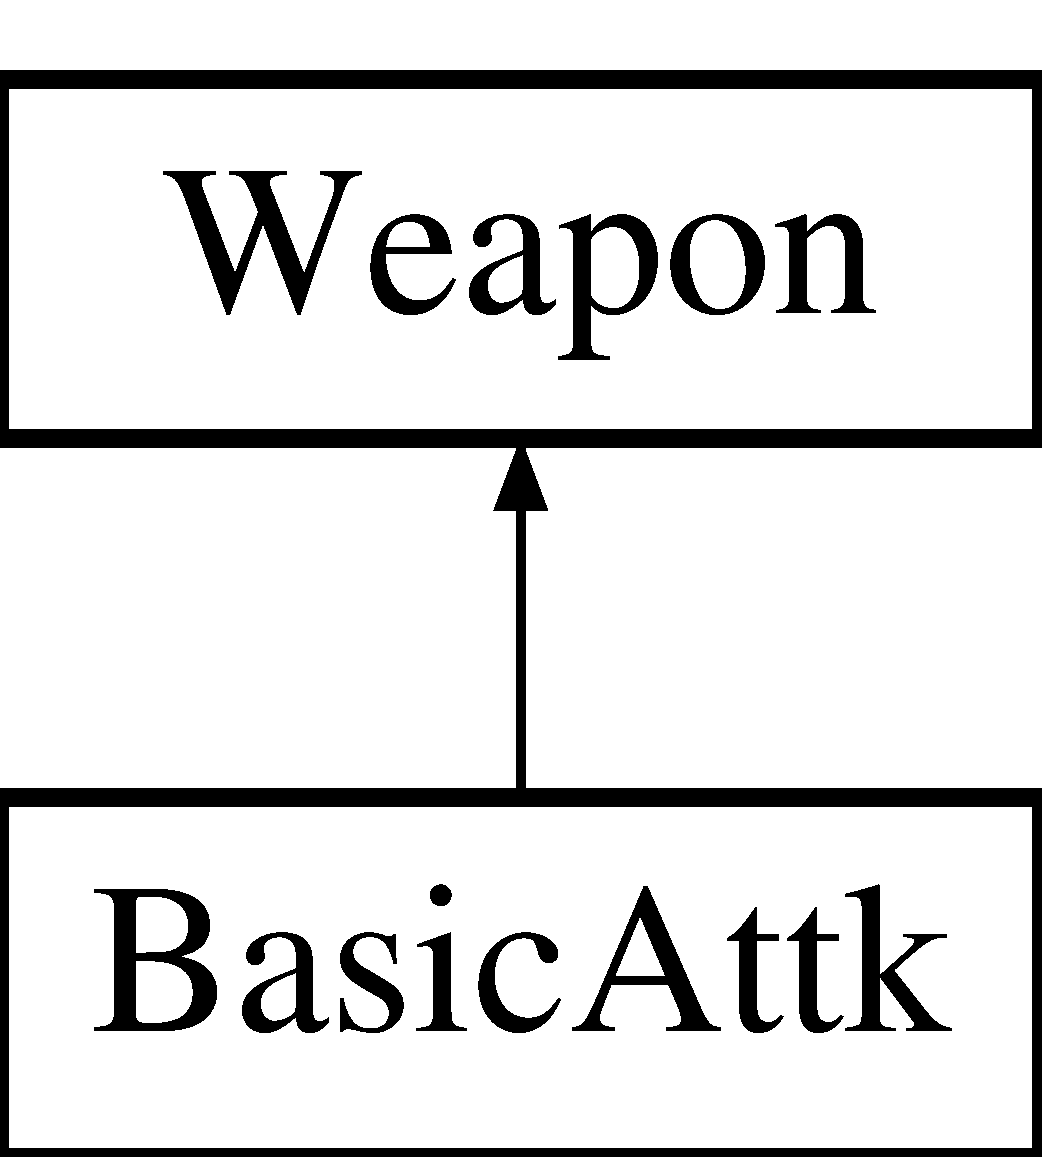
\includegraphics[height=2cm]{classBasicAttk}
\end{center}
\end{figure}
\subsection*{Public Member Functions}
\begin{DoxyCompactItemize}
\item 
\hypertarget{classBasicAttk_afea1d0e3a36bb57427a0d5c01e8b54b1}{
\hyperlink{classBasicAttk_afea1d0e3a36bb57427a0d5c01e8b54b1}{BasicAttk} ()}
\label{classBasicAttk_afea1d0e3a36bb57427a0d5c01e8b54b1}

\begin{DoxyCompactList}\small\item\em Constructors and Destructors. \item\end{DoxyCompactList}\item 
void \hyperlink{classBasicAttk_a1c717fc7e6060ec94764adb1743f7ee4}{attack} (\hyperlink{classCharacter}{Character} $\ast$attacker, \hyperlink{classCharacter}{Character} $\ast$who)
\end{DoxyCompactItemize}


\subsection{Member Function Documentation}
\hypertarget{classBasicAttk_a1c717fc7e6060ec94764adb1743f7ee4}{
\index{BasicAttk@{BasicAttk}!attack@{attack}}
\index{attack@{attack}!BasicAttk@{BasicAttk}}
\subsubsection[{attack}]{\setlength{\rightskip}{0pt plus 5cm}void BasicAttk::attack ({\bf Character} $\ast$ {\em attacker}, \/  {\bf Character} $\ast$ {\em who})\hspace{0.3cm}{\ttfamily  \mbox{[}virtual\mbox{]}}}}
\label{classBasicAttk_a1c717fc7e6060ec94764adb1743f7ee4}
Attack method that takes in an attacker and who will be attacked \hyperlink{classCharacter}{Character} objects Who will be damaged by the attackDamage of \hyperlink{classBasicAttk}{BasicAttk} Attacker receives counter damage equal to half the attackDamage Outputs to the screen what happens 

Implements \hyperlink{classWeapon_a74d99dd40d8872718710bcf94fff98d7}{Weapon}.

The documentation for this class was generated from the following files:\begin{DoxyCompactItemize}
\item 
Weapon.h\item 
Weapon.cpp\end{DoxyCompactItemize}

\hypertarget{classBomb}{
\section{Bomb Class Reference}
\label{classBomb}\index{Bomb@{Bomb}}
}
Inheritance diagram for Bomb::\begin{figure}[H]
\begin{center}
\leavevmode
\includegraphics[height=2cm]{classBomb}
\end{center}
\end{figure}
\subsection*{Public Member Functions}
\begin{DoxyCompactItemize}
\item 
\hypertarget{classBomb_a5805401b6cfbb451cf31ebd4851740cf}{
\hyperlink{classBomb_a5805401b6cfbb451cf31ebd4851740cf}{Bomb} ()}
\label{classBomb_a5805401b6cfbb451cf31ebd4851740cf}

\begin{DoxyCompactList}\small\item\em Constructors and Destructors. \item\end{DoxyCompactList}\item 
\hypertarget{classBomb_a7756be7b4e8425c84b27f98b39624b59}{
std::string \hyperlink{classBomb_a7756be7b4e8425c84b27f98b39624b59}{getName} () const }
\label{classBomb_a7756be7b4e8425c84b27f98b39624b59}

\begin{DoxyCompactList}\small\item\em Retrieves the name of the item. \item\end{DoxyCompactList}\item 
\hypertarget{classBomb_a24f4bc2a846224e23a3e0a9ebd7011ee}{
int \hyperlink{classBomb_a24f4bc2a846224e23a3e0a9ebd7011ee}{getQuantity} () const }
\label{classBomb_a24f4bc2a846224e23a3e0a9ebd7011ee}

\begin{DoxyCompactList}\small\item\em Retries the quantity of Bombs. \item\end{DoxyCompactList}\item 
void \hyperlink{classBomb_ae0472ffdfeb98f780e8c63967d4e81ed}{useItem} (\hyperlink{classPlayer}{Player} $\ast$who)
\item 
\hypertarget{classBomb_aea5f2bb72dec8d3c9346bd9398ab4eaa}{
void \hyperlink{classBomb_aea5f2bb72dec8d3c9346bd9398ab4eaa}{increment} ()}
\label{classBomb_aea5f2bb72dec8d3c9346bd9398ab4eaa}

\begin{DoxyCompactList}\small\item\em Increase the quantity of Bombs. \item\end{DoxyCompactList}\end{DoxyCompactItemize}


\subsection{Member Function Documentation}
\hypertarget{classBomb_ae0472ffdfeb98f780e8c63967d4e81ed}{
\index{Bomb@{Bomb}!useItem@{useItem}}
\index{useItem@{useItem}!Bomb@{Bomb}}
\subsubsection[{useItem}]{\setlength{\rightskip}{0pt plus 5cm}void Bomb::useItem ({\bf Player} $\ast$ {\em who})\hspace{0.3cm}{\ttfamily  \mbox{[}virtual\mbox{]}}}}
\label{classBomb_ae0472ffdfeb98f780e8c63967d4e81ed}
Method that use the item on the player object that is passed into it, logic for the bomb is done in here Decreases quantity of item 

Implements \hyperlink{classItems}{Items}.

The documentation for this class was generated from the following files:\begin{DoxyCompactItemize}
\item 
Items.h\item 
Items.cpp\end{DoxyCompactItemize}

\hypertarget{classCastle}{
\section{Castle Class Reference}
\label{classCastle}\index{Castle@{Castle}}
}


{\ttfamily \#include $<$Castle.h$>$}Inheritance diagram for Castle::\begin{figure}[H]
\begin{center}
\leavevmode
\includegraphics[height=2cm]{classCastle}
\end{center}
\end{figure}
\subsection*{Public Member Functions}
\begin{DoxyCompactItemize}
\item 
\hypertarget{classCastle_ab5a57307b5e4c8ecb6f8f0524684e6d6}{
\hyperlink{classCastle_ab5a57307b5e4c8ecb6f8f0524684e6d6}{Castle} ()}
\label{classCastle_ab5a57307b5e4c8ecb6f8f0524684e6d6}

\begin{DoxyCompactList}\small\item\em Constructors and Destructors. \item\end{DoxyCompactList}\item 
void \hyperlink{classCastle_a4a961593bd68b77a7839d31da9d8dcd6}{run} (\hyperlink{classPlayer}{Player} $\ast$player)
\begin{DoxyCompactList}\small\item\em The class that will run the entire \hyperlink{classCave}{Cave} environment, sets up the enemies, and designates what happens in this time. \item\end{DoxyCompactList}\end{DoxyCompactItemize}


\subsection{Detailed Description}
The class represnets a \hyperlink{classCastle}{Castle} 

\subsection{Member Function Documentation}
\hypertarget{classCastle_a4a961593bd68b77a7839d31da9d8dcd6}{
\index{Castle@{Castle}!run@{run}}
\index{run@{run}!Castle@{Castle}}
\subsubsection[{run}]{\setlength{\rightskip}{0pt plus 5cm}void Castle::run ({\bf Player} $\ast$ {\em p})\hspace{0.3cm}{\ttfamily  \mbox{[}virtual\mbox{]}}}}
\label{classCastle_a4a961593bd68b77a7839d31da9d8dcd6}


The class that will run the entire \hyperlink{classCave}{Cave} environment, sets up the enemies, and designates what happens in this time. This method executes the logics of the \hyperlink{classCastle}{Castle} chapter 

Implements \hyperlink{classEnviros}{Enviros}.

The documentation for this class was generated from the following files:\begin{DoxyCompactItemize}
\item 
Castle.h\item 
Castle.cpp\end{DoxyCompactItemize}

\hypertarget{classCave}{
\section{Cave Class Reference}
\label{classCave}\index{Cave@{Cave}}
}


{\ttfamily \#include $<$Cave.h$>$}Inheritance diagram for Cave::\begin{figure}[H]
\begin{center}
\leavevmode
\includegraphics[height=2cm]{classCave}
\end{center}
\end{figure}
\subsection*{Public Member Functions}
\begin{DoxyCompactItemize}
\item 
\hypertarget{classCave_a3521990d4fcc6d69e70e31f0c74bef12}{
\hyperlink{classCave_a3521990d4fcc6d69e70e31f0c74bef12}{Cave} ()}
\label{classCave_a3521990d4fcc6d69e70e31f0c74bef12}

\begin{DoxyCompactList}\small\item\em Constructors and Destructors. \item\end{DoxyCompactList}\item 
void \hyperlink{classCave_a64da68a2408b66f8222f087e600bbdcf}{run} (\hyperlink{classPlayer}{Player} $\ast$player)
\begin{DoxyCompactList}\small\item\em The class that will run the entire \hyperlink{classCave}{Cave} environment, sets up the enemies, and designates what happens in this time. \item\end{DoxyCompactList}\end{DoxyCompactItemize}


\subsection{Detailed Description}
The class represnets a \hyperlink{classForest}{Forest} 

\subsection{Member Function Documentation}
\hypertarget{classCave_a64da68a2408b66f8222f087e600bbdcf}{
\index{Cave@{Cave}!run@{run}}
\index{run@{run}!Cave@{Cave}}
\subsubsection[{run}]{\setlength{\rightskip}{0pt plus 5cm}void Cave::run ({\bf Player} $\ast$ {\em p})\hspace{0.3cm}{\ttfamily  \mbox{[}virtual\mbox{]}}}}
\label{classCave_a64da68a2408b66f8222f087e600bbdcf}


The class that will run the entire \hyperlink{classCave}{Cave} environment, sets up the enemies, and designates what happens in this time. This method executes the logics of the \hyperlink{classCave}{Cave} chapter 

Implements \hyperlink{classEnviros}{Enviros}.

The documentation for this class was generated from the following files:\begin{DoxyCompactItemize}
\item 
Cave.h\item 
Cave.cpp\end{DoxyCompactItemize}

\hypertarget{classCharacter}{
\section{Character Class Reference}
\label{classCharacter}\index{Character@{Character}}
}
Inheritance diagram for Character::\begin{figure}[H]
\begin{center}
\leavevmode
\includegraphics[height=2cm]{classCharacter}
\end{center}
\end{figure}
\subsection*{Public Member Functions}
\begin{DoxyCompactItemize}
\item 
\hypertarget{classCharacter_a0b0509282cf2dbb4a2aed19d2226ab16}{
\hyperlink{classCharacter_a0b0509282cf2dbb4a2aed19d2226ab16}{Character} (const std::string CharacterName)}
\label{classCharacter_a0b0509282cf2dbb4a2aed19d2226ab16}

\begin{DoxyCompactList}\small\item\em Constructors and Destructors. \item\end{DoxyCompactList}\item 
\hypertarget{classCharacter_a95a6a763b1f9ea188899ea63bb24f659}{
{\bfseries Character} (const std::string CharacterName, int h)}
\label{classCharacter_a95a6a763b1f9ea188899ea63bb24f659}

\item 
\hypertarget{classCharacter_a541f9063682bf9f9714702e7ffb2e64c}{
std::string \hyperlink{classCharacter_a541f9063682bf9f9714702e7ffb2e64c}{getName} () const }
\label{classCharacter_a541f9063682bf9f9714702e7ffb2e64c}

\begin{DoxyCompactList}\small\item\em Getters and Setters. \item\end{DoxyCompactList}\item 
\hypertarget{classCharacter_a9f3a54d21fb6c88cdebbc7bf29a9cab7}{
void \hyperlink{classCharacter_a9f3a54d21fb6c88cdebbc7bf29a9cab7}{setName} (std::string n)}
\label{classCharacter_a9f3a54d21fb6c88cdebbc7bf29a9cab7}

\begin{DoxyCompactList}\small\item\em Sets the name. \item\end{DoxyCompactList}\item 
\hypertarget{classCharacter_aa49f985b1b05751b2d4b3de74b4acc8c}{
bool \hyperlink{classCharacter_aa49f985b1b05751b2d4b3de74b4acc8c}{isAlive} ()}
\label{classCharacter_aa49f985b1b05751b2d4b3de74b4acc8c}

\begin{DoxyCompactList}\small\item\em Checks to see if the \hyperlink{classCharacter}{Character} is alive, returns true or false. \item\end{DoxyCompactList}\item 
\hypertarget{classCharacter_a5b708af3b8b185fd694722c7a566a4a7}{
void \hyperlink{classCharacter_a5b708af3b8b185fd694722c7a566a4a7}{kill} ()}
\label{classCharacter_a5b708af3b8b185fd694722c7a566a4a7}

\begin{DoxyCompactList}\small\item\em Kills the character and sets its health to 0. \item\end{DoxyCompactList}\item 
\hypertarget{classCharacter_a216657cde7bd88523bbeb3ae3abffd31}{
void \hyperlink{classCharacter_a216657cde7bd88523bbeb3ae3abffd31}{dropHealth} (int amount)}
\label{classCharacter_a216657cde7bd88523bbeb3ae3abffd31}

\begin{DoxyCompactList}\small\item\em Drops the health of the character by the amount of the integer specified. \item\end{DoxyCompactList}\item 
\hypertarget{classCharacter_a64fd5a2b59913c1b01dfaa43e3729987}{
void {\bfseries increaseHealth} (int amount)}
\label{classCharacter_a64fd5a2b59913c1b01dfaa43e3729987}

\item 
\hypertarget{classCharacter_af1e08fcaa1002081fc729dd3101db049}{
int \hyperlink{classCharacter_af1e08fcaa1002081fc729dd3101db049}{getHealth} () const }
\label{classCharacter_af1e08fcaa1002081fc729dd3101db049}

\begin{DoxyCompactList}\small\item\em Return the health of the \hyperlink{classCharacter}{Character} as an integer. \item\end{DoxyCompactList}\item 
\hypertarget{classCharacter_ad717effc421d6300edccdff2d3dec35a}{
void \hyperlink{classCharacter_ad717effc421d6300edccdff2d3dec35a}{printHealth} () const }
\label{classCharacter_ad717effc421d6300edccdff2d3dec35a}

\begin{DoxyCompactList}\small\item\em Prints the health of the \hyperlink{classCharacter}{Character} to the screen. \item\end{DoxyCompactList}\end{DoxyCompactItemize}


The documentation for this class was generated from the following files:\begin{DoxyCompactItemize}
\item 
Character.h\item 
Character.cpp\end{DoxyCompactItemize}

\hypertarget{classEnemy}{
\section{Enemy Class Reference}
\label{classEnemy}\index{Enemy@{Enemy}}
}
Inheritance diagram for Enemy::\begin{figure}[H]
\begin{center}
\leavevmode
\includegraphics[height=2cm]{classEnemy}
\end{center}
\end{figure}
\subsection*{Public Member Functions}
\begin{DoxyCompactItemize}
\item 
\hypertarget{classEnemy_a3bd848647f3dbab14f8ccf6ecb1a1f17}{
\hyperlink{classEnemy_a3bd848647f3dbab14f8ccf6ecb1a1f17}{Enemy} (const std::string enemyName, int h)}
\label{classEnemy_a3bd848647f3dbab14f8ccf6ecb1a1f17}

\begin{DoxyCompactList}\small\item\em Constructors and Destructors. \item\end{DoxyCompactList}\item 
\hypertarget{classEnemy_a9242db04b8819769567ea7ac831a3081}{
{\bfseries Enemy} (const std::string enemyName, int h, \hyperlink{classItems}{Items} $\ast$i)}
\label{classEnemy_a9242db04b8819769567ea7ac831a3081}

\item 
\hypertarget{classEnemy_a4a2abf29b609f61de397f7b87e9e9085}{
\hyperlink{classPlayer}{Player} $\ast$ \hyperlink{classEnemy_a4a2abf29b609f61de397f7b87e9e9085}{giveItem} (\hyperlink{classPlayer}{Player} $\ast$who)}
\label{classEnemy_a4a2abf29b609f61de397f7b87e9e9085}

\begin{DoxyCompactList}\small\item\em This passes the object \_\-item that the \hyperlink{classEnemy}{Enemy} has and gives it to the \hyperlink{classPlayer}{Player} object. \item\end{DoxyCompactList}\end{DoxyCompactItemize}


The documentation for this class was generated from the following files:\begin{DoxyCompactItemize}
\item 
Enemy.h\item 
Enemy.cpp\end{DoxyCompactItemize}

\hypertarget{classEnviros}{
\section{Enviros Class Reference}
\label{classEnviros}\index{Enviros@{Enviros}}
}
Inheritance diagram for Enviros::\begin{figure}[H]
\begin{center}
\leavevmode
\includegraphics[height=2cm]{classEnviros}
\end{center}
\end{figure}
\subsection*{Public Member Functions}
\begin{DoxyCompactItemize}
\item 
\hypertarget{classEnviros_a92754322cdad0af0e9d74fee0b1b6ce1}{
\hyperlink{classEnviros_a92754322cdad0af0e9d74fee0b1b6ce1}{Enviros} ()}
\label{classEnviros_a92754322cdad0af0e9d74fee0b1b6ce1}

\begin{DoxyCompactList}\small\item\em Constructors and Destructors. \item\end{DoxyCompactList}\item 
\hypertarget{classEnviros_a832d9de2546c75cc92f4fe447f907ece}{
virtual void {\bfseries run} (\hyperlink{classPlayer}{Player} $\ast$player)=0}
\label{classEnviros_a832d9de2546c75cc92f4fe447f907ece}

\item 
\hypertarget{classEnviros_a87473892a35835256edbe83972869a06}{
void \hyperlink{classEnviros_a87473892a35835256edbe83972869a06}{printInstruction} ()}
\label{classEnviros_a87473892a35835256edbe83972869a06}

\begin{DoxyCompactList}\small\item\em Prints the instructions and options for a battle sequence. \item\end{DoxyCompactList}\item 
\hypertarget{classEnviros_aade391c233eb14d53e2db1aca3abe837}{
void \hyperlink{classEnviros_aade391c233eb14d53e2db1aca3abe837}{printEnviroInstruct} ()}
\label{classEnviros_aade391c233eb14d53e2db1aca3abe837}

\begin{DoxyCompactList}\small\item\em Prints the instructions and options when in the environment. \item\end{DoxyCompactList}\end{DoxyCompactItemize}


The documentation for this class was generated from the following files:\begin{DoxyCompactItemize}
\item 
Enviros.h\item 
Enviros.cpp\end{DoxyCompactItemize}

\hypertarget{classFireAttk}{
\section{FireAttk Class Reference}
\label{classFireAttk}\index{FireAttk@{FireAttk}}
}
Inheritance diagram for FireAttk::\begin{figure}[H]
\begin{center}
\leavevmode
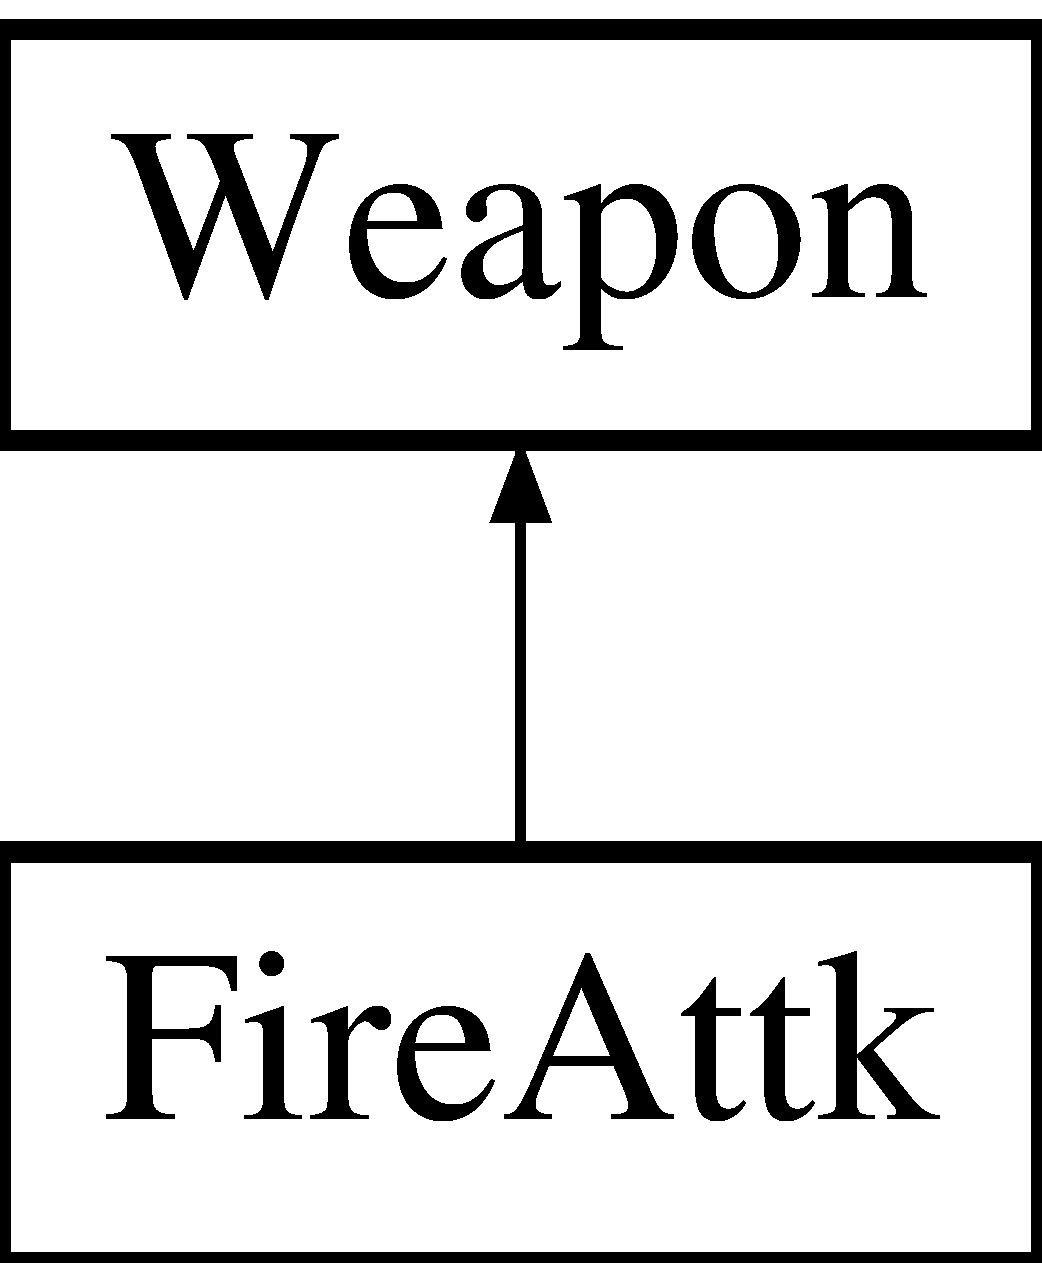
\includegraphics[height=2cm]{classFireAttk}
\end{center}
\end{figure}
\subsection*{Public Member Functions}
\begin{DoxyCompactItemize}
\item 
\hypertarget{classFireAttk_abec5fb6b60d210f2633ba0ac0ecea017}{
\hyperlink{classFireAttk_abec5fb6b60d210f2633ba0ac0ecea017}{FireAttk} ()}
\label{classFireAttk_abec5fb6b60d210f2633ba0ac0ecea017}

\begin{DoxyCompactList}\small\item\em Constructors and Destructors. \item\end{DoxyCompactList}\item 
void \hyperlink{classFireAttk_a0a6f02e6cb56e5ceabde1fff79be7dd4}{attack} (\hyperlink{classCharacter}{Character} $\ast$attacker, \hyperlink{classCharacter}{Character} $\ast$who)
\end{DoxyCompactItemize}


\subsection{Member Function Documentation}
\hypertarget{classFireAttk_a0a6f02e6cb56e5ceabde1fff79be7dd4}{
\index{FireAttk@{FireAttk}!attack@{attack}}
\index{attack@{attack}!FireAttk@{FireAttk}}
\subsubsection[{attack}]{\setlength{\rightskip}{0pt plus 5cm}void FireAttk::attack ({\bf Character} $\ast$ {\em attacker}, \/  {\bf Character} $\ast$ {\em who})\hspace{0.3cm}{\ttfamily  \mbox{[}virtual\mbox{]}}}}
\label{classFireAttk_a0a6f02e6cb56e5ceabde1fff79be7dd4}
Attack method that takes in an attacker and who will be attacked \hyperlink{classCharacter}{Character} objects Who will be damaged by the attackDamage of \hyperlink{classFireAttk}{FireAttk} Attacker receives counter damage equal to half the attackDamage Outputs to the screen what happens 

Implements \hyperlink{classWeapon_a74d99dd40d8872718710bcf94fff98d7}{Weapon}.

The documentation for this class was generated from the following files:\begin{DoxyCompactItemize}
\item 
Weapon.h\item 
Weapon.cpp\end{DoxyCompactItemize}

\hypertarget{classForest}{
\section{Forest Class Reference}
\label{classForest}\index{Forest@{Forest}}
}


{\ttfamily \#include $<$Forest.h$>$}Inheritance diagram for Forest::\begin{figure}[H]
\begin{center}
\leavevmode
\includegraphics[height=2cm]{classForest}
\end{center}
\end{figure}
\subsection*{Public Member Functions}
\begin{DoxyCompactItemize}
\item 
\hypertarget{classForest_af9ad2787ae306cb4da8d7443da124d15}{
\hyperlink{classForest_af9ad2787ae306cb4da8d7443da124d15}{Forest} ()}
\label{classForest_af9ad2787ae306cb4da8d7443da124d15}

\begin{DoxyCompactList}\small\item\em Constructors and Destructors. \item\end{DoxyCompactList}\item 
void \hyperlink{classForest_a22996cfd5e18402e640316b7a6fb5feb}{run} (\hyperlink{classPlayer}{Player} $\ast$player)
\begin{DoxyCompactList}\small\item\em The class that will run the entire \hyperlink{classCave}{Cave} environment, sets up the enemies, and designates what happens in this time. \item\end{DoxyCompactList}\end{DoxyCompactItemize}


\subsection{Detailed Description}
The class represnets a \hyperlink{classForest}{Forest} 

\subsection{Member Function Documentation}
\hypertarget{classForest_a22996cfd5e18402e640316b7a6fb5feb}{
\index{Forest@{Forest}!run@{run}}
\index{run@{run}!Forest@{Forest}}
\subsubsection[{run}]{\setlength{\rightskip}{0pt plus 5cm}void Forest::run ({\bf Player} $\ast$ {\em p})\hspace{0.3cm}{\ttfamily  \mbox{[}virtual\mbox{]}}}}
\label{classForest_a22996cfd5e18402e640316b7a6fb5feb}


The class that will run the entire \hyperlink{classCave}{Cave} environment, sets up the enemies, and designates what happens in this time. This method executes the logics of the \hyperlink{classForest}{Forest} chapter 

Implements \hyperlink{classEnviros}{Enviros}.

The documentation for this class was generated from the following files:\begin{DoxyCompactItemize}
\item 
Forest.h\item 
Forest.cpp\end{DoxyCompactItemize}

\hypertarget{classIceAttk}{
\section{IceAttk Class Reference}
\label{classIceAttk}\index{IceAttk@{IceAttk}}
}
Inheritance diagram for IceAttk::\begin{figure}[H]
\begin{center}
\leavevmode
\includegraphics[height=2cm]{classIceAttk}
\end{center}
\end{figure}
\subsection*{Public Member Functions}
\begin{DoxyCompactItemize}
\item 
\hypertarget{classIceAttk_a02184f028f162a82bd97e0ef14c027f6}{
\hyperlink{classIceAttk_a02184f028f162a82bd97e0ef14c027f6}{IceAttk} ()}
\label{classIceAttk_a02184f028f162a82bd97e0ef14c027f6}

\begin{DoxyCompactList}\small\item\em Constructors and Destructors. \item\end{DoxyCompactList}\item 
void \hyperlink{classIceAttk_a4284b30231a9881ebc34fc3e01cc17cc}{attack} (\hyperlink{classCharacter}{Character} $\ast$attacker, \hyperlink{classCharacter}{Character} $\ast$who)
\end{DoxyCompactItemize}


\subsection{Member Function Documentation}
\hypertarget{classIceAttk_a4284b30231a9881ebc34fc3e01cc17cc}{
\index{IceAttk@{IceAttk}!attack@{attack}}
\index{attack@{attack}!IceAttk@{IceAttk}}
\subsubsection[{attack}]{\setlength{\rightskip}{0pt plus 5cm}void IceAttk::attack ({\bf Character} $\ast$ {\em attacker}, \/  {\bf Character} $\ast$ {\em who})\hspace{0.3cm}{\ttfamily  \mbox{[}virtual\mbox{]}}}}
\label{classIceAttk_a4284b30231a9881ebc34fc3e01cc17cc}
Attack method that takes in an attacker and who will be attacked \hyperlink{classCharacter}{Character} objects Who will be damaged by the attackDamage of \hyperlink{classIceAttk}{IceAttk} Attacker receives counter damage equal to half the attackDamage Outputs to the screen what happens 

Implements \hyperlink{classWeapon_a74d99dd40d8872718710bcf94fff98d7}{Weapon}.

The documentation for this class was generated from the following files:\begin{DoxyCompactItemize}
\item 
Weapon.h\item 
Weapon.cpp\end{DoxyCompactItemize}

\hypertarget{classinvalid__input}{
\section{invalid\_\-input Class Reference}
\label{classinvalid__input}\index{invalid\_\-input@{invalid\_\-input}}
}
\subsection*{Public Member Functions}
\begin{DoxyCompactItemize}
\item 
\hypertarget{classinvalid__input_ad4945c86eaa7eb9470bdfc23e7ea2fb9}{
{\bfseries invalid\_\-coordinates\_\-error} (const std::string \&what\_\-arg)}
\label{classinvalid__input_ad4945c86eaa7eb9470bdfc23e7ea2fb9}

\item 
\hypertarget{classinvalid__input_aafb8b5281994c883712f7be6fc2f6b00}{
virtual const char $\ast$ {\bfseries what} () const   throw ()}
\label{classinvalid__input_aafb8b5281994c883712f7be6fc2f6b00}

\end{DoxyCompactItemize}


The documentation for this class was generated from the following files:\begin{DoxyCompactItemize}
\item 
Exceptions.h\item 
Exceptions.cpp\end{DoxyCompactItemize}

\hypertarget{classinvalid__move__error}{
\section{invalid\_\-move\_\-error Class Reference}
\label{classinvalid__move__error}\index{invalid\_\-move\_\-error@{invalid\_\-move\_\-error}}
}
\subsection*{Public Member Functions}
\begin{DoxyCompactItemize}
\item 
\hypertarget{classinvalid__move__error_adc9a651482c3b4469a2798eb2c382d46}{
{\bfseries invalid\_\-move\_\-error} (const std::string \&what\_\-arg)}
\label{classinvalid__move__error_adc9a651482c3b4469a2798eb2c382d46}

\item 
\hypertarget{classinvalid__move__error_ac91c3fcf1ac791269ae1b6eb0aa5603d}{
virtual const char $\ast$ {\bfseries what} () const   throw ()}
\label{classinvalid__move__error_ac91c3fcf1ac791269ae1b6eb0aa5603d}

\end{DoxyCompactItemize}


The documentation for this class was generated from the following files:\begin{DoxyCompactItemize}
\item 
Exceptions.h\item 
Exceptions.cpp\end{DoxyCompactItemize}

\hypertarget{classItems}{
\section{Items Class Reference}
\label{classItems}\index{Items@{Items}}
}
Inheritance diagram for Items::\begin{figure}[H]
\begin{center}
\leavevmode
\includegraphics[height=2cm]{classItems}
\end{center}
\end{figure}
\subsection*{Public Member Functions}
\begin{DoxyCompactItemize}
\item 
\hypertarget{classItems_a3d368c3c7a14eb2a038682bd4da5d41a}{
\hyperlink{classItems_a3d368c3c7a14eb2a038682bd4da5d41a}{Items} ()}
\label{classItems_a3d368c3c7a14eb2a038682bd4da5d41a}

\begin{DoxyCompactList}\small\item\em Constructors and Destructors. \item\end{DoxyCompactList}\item 
\hypertarget{classItems_aa61eb1d6a814abd395776a5f4b63282b}{
virtual std::string \hyperlink{classItems_aa61eb1d6a814abd395776a5f4b63282b}{getName} () const =0}
\label{classItems_aa61eb1d6a814abd395776a5f4b63282b}

\begin{DoxyCompactList}\small\item\em Pure virtual methods. \item\end{DoxyCompactList}\item 
\hypertarget{classItems_ab575aac56a555d99ec836c792559a485}{
virtual int {\bfseries getQuantity} () const =0}
\label{classItems_ab575aac56a555d99ec836c792559a485}

\item 
\hypertarget{classItems_a6e315b13ab669be1cc37e23f185c6d0b}{
virtual void {\bfseries useItem} (\hyperlink{classPlayer}{Player} $\ast$who)=0}
\label{classItems_a6e315b13ab669be1cc37e23f185c6d0b}

\item 
\hypertarget{classItems_a70e74576f122eab10323537dede2de6e}{
virtual void {\bfseries increment} ()=0}
\label{classItems_a70e74576f122eab10323537dede2de6e}

\end{DoxyCompactItemize}


The documentation for this class was generated from the following file:\begin{DoxyCompactItemize}
\item 
Items.h\end{DoxyCompactItemize}

\hypertarget{classLandofTorvold}{
\section{LandofTorvold Class Reference}
\label{classLandofTorvold}\index{LandofTorvold@{LandofTorvold}}
}


{\ttfamily \#include $<$LandofTorvold.h$>$}\subsection*{Public Member Functions}
\begin{DoxyCompactItemize}
\item 
\hypertarget{classLandofTorvold_a1f23bf2996aeda2defaa5ba2e8a4e3e5}{
\hyperlink{classLandofTorvold_a1f23bf2996aeda2defaa5ba2e8a4e3e5}{LandofTorvold} ()}
\label{classLandofTorvold_a1f23bf2996aeda2defaa5ba2e8a4e3e5}

\begin{DoxyCompactList}\small\item\em Constructors and Destructors. \item\end{DoxyCompactList}\item 
\hypertarget{classLandofTorvold_acfc219cfc76280f6394ad416e3bf748f}{
void \hyperlink{classLandofTorvold_acfc219cfc76280f6394ad416e3bf748f}{run} ()}
\label{classLandofTorvold_acfc219cfc76280f6394ad416e3bf748f}

\begin{DoxyCompactList}\small\item\em Runs the Land of Torvold controller class that invokes the other environment's run classes. \item\end{DoxyCompactList}\end{DoxyCompactItemize}


\subsection{Detailed Description}
This represents the class that will run the whole game 

The documentation for this class was generated from the following files:\begin{DoxyCompactItemize}
\item 
LandofTorvold.h\item 
LandofTorvold.cpp\end{DoxyCompactItemize}

\hypertarget{classMasterSword}{
\section{MasterSword Class Reference}
\label{classMasterSword}\index{MasterSword@{MasterSword}}
}
Inheritance diagram for MasterSword::\begin{figure}[H]
\begin{center}
\leavevmode
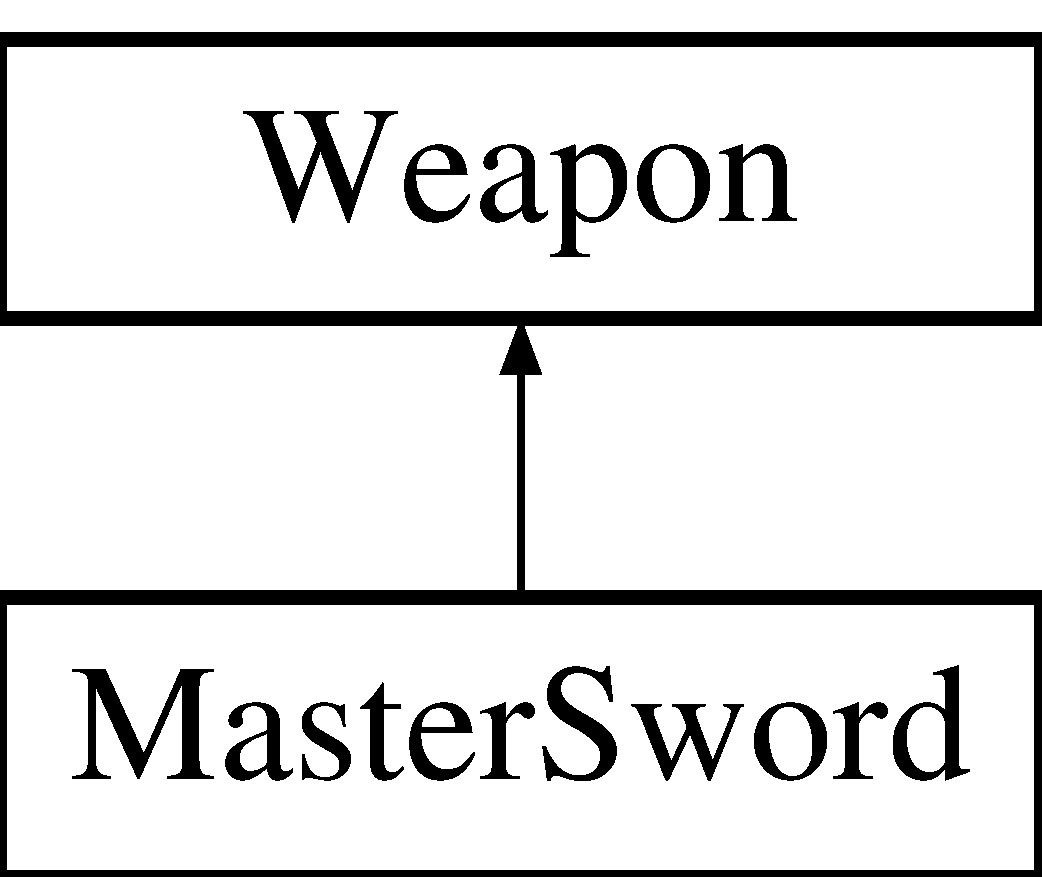
\includegraphics[height=2cm]{classMasterSword}
\end{center}
\end{figure}
\subsection*{Public Member Functions}
\begin{DoxyCompactItemize}
\item 
\hypertarget{classMasterSword_a032920b9abdd54a80efc69c81c90900d}{
\hyperlink{classMasterSword_a032920b9abdd54a80efc69c81c90900d}{MasterSword} ()}
\label{classMasterSword_a032920b9abdd54a80efc69c81c90900d}

\begin{DoxyCompactList}\small\item\em Constructors and Destructors. \item\end{DoxyCompactList}\item 
void \hyperlink{classMasterSword_ac407c8f47fdcb95d8404a33aed004358}{attack} (\hyperlink{classCharacter}{Character} $\ast$attacker, \hyperlink{classCharacter}{Character} $\ast$who)
\end{DoxyCompactItemize}


\subsection{Member Function Documentation}
\hypertarget{classMasterSword_ac407c8f47fdcb95d8404a33aed004358}{
\index{MasterSword@{MasterSword}!attack@{attack}}
\index{attack@{attack}!MasterSword@{MasterSword}}
\subsubsection[{attack}]{\setlength{\rightskip}{0pt plus 5cm}void MasterSword::attack ({\bf Character} $\ast$ {\em attacker}, \/  {\bf Character} $\ast$ {\em who})\hspace{0.3cm}{\ttfamily  \mbox{[}virtual\mbox{]}}}}
\label{classMasterSword_ac407c8f47fdcb95d8404a33aed004358}
Attack method that takes in an attacker and who will be attacked \hyperlink{classCharacter}{Character} objects Who will be damaged by the attackDamage of \hyperlink{classMasterSword}{MasterSword} Attacker receives counter damage equal to half the attackDamage Outputs to the screen what happens 

Implements \hyperlink{classWeapon_a74d99dd40d8872718710bcf94fff98d7}{Weapon}.

The documentation for this class was generated from the following files:\begin{DoxyCompactItemize}
\item 
Weapon.h\item 
Weapon.cpp\end{DoxyCompactItemize}

\hypertarget{classPlayer}{
\section{Player Class Reference}
\label{classPlayer}\index{Player@{Player}}
}


{\ttfamily \#include $<$Player.h$>$}Inheritance diagram for Player::\begin{figure}[H]
\begin{center}
\leavevmode
\includegraphics[height=2cm]{classPlayer}
\end{center}
\end{figure}
\subsection*{Public Member Functions}
\begin{DoxyCompactItemize}
\item 
\hyperlink{classPlayer_a8d83d0f0e6ff61b2003b9769c8be3f88}{Player} (const string playerName)
\begin{DoxyCompactList}\small\item\em Constructors and Destructors. \item\end{DoxyCompactList}\item 
\hyperlink{classPlayer_a25291eed6de2d4ffe9f72422c79af64c}{Player} (const string playerName, int h)
\item 
\hypertarget{classPlayer_a5eabedb92d98c4b70fa2b1882404f058}{
void \hyperlink{classPlayer_a5eabedb92d98c4b70fa2b1882404f058}{addItem} (\hyperlink{classItems}{Items} $\ast$i)}
\label{classPlayer_a5eabedb92d98c4b70fa2b1882404f058}

\begin{DoxyCompactList}\small\item\em Adds an item of type object to the \hyperlink{classPlayer}{Player} by incremeting the quantity of that specific item in its itemList. \item\end{DoxyCompactList}\item 
\hypertarget{classPlayer_a704c8bad5a62ecf3a0e07a091380ff58}{
void \hyperlink{classPlayer_a704c8bad5a62ecf3a0e07a091380ff58}{useItem} (\hyperlink{classItems}{Items} $\ast$i)}
\label{classPlayer_a704c8bad5a62ecf3a0e07a091380ff58}

\begin{DoxyCompactList}\small\item\em Uses an item by calling the useItem method in its appropriate position in the vector itemList. \item\end{DoxyCompactList}\item 
\hypertarget{classPlayer_a896a4cdfdc5f616c32e5b2ac2cb6b72f}{
vector$<$ \hyperlink{classItems}{Items} $\ast$ $>$ \hyperlink{classPlayer_a896a4cdfdc5f616c32e5b2ac2cb6b72f}{getInventory} () const }
\label{classPlayer_a896a4cdfdc5f616c32e5b2ac2cb6b72f}

\begin{DoxyCompactList}\small\item\em Returns the Vector of items available to the \hyperlink{classPlayer}{Player}. \item\end{DoxyCompactList}\item 
\hypertarget{classPlayer_a70d4c5eb304121aaa606569d522cf1ba}{
void \hyperlink{classPlayer_a70d4c5eb304121aaa606569d522cf1ba}{showItems} () const }
\label{classPlayer_a70d4c5eb304121aaa606569d522cf1ba}

\begin{DoxyCompactList}\small\item\em Outputs the items and their quantities to the screen. \item\end{DoxyCompactList}\item 
\hypertarget{classPlayer_a933947160a754eebca73275b8d45ae38}{
void \hyperlink{classPlayer_a933947160a754eebca73275b8d45ae38}{attack} (\hyperlink{classCharacter}{Character} $\ast$who)}
\label{classPlayer_a933947160a754eebca73275b8d45ae38}

\begin{DoxyCompactList}\small\item\em Attack method that passes who will be attacked. \item\end{DoxyCompactList}\item 
\hypertarget{classPlayer_a0c4b8585e95d3092ec4d0f852091f12a}{
void \hyperlink{classPlayer_a0c4b8585e95d3092ec4d0f852091f12a}{setWeapon} (\hyperlink{classWeapon}{Weapon} $\ast$weaponType)}
\label{classPlayer_a0c4b8585e95d3092ec4d0f852091f12a}

\begin{DoxyCompactList}\small\item\em Sets the weaponType of the \hyperlink{classPlayer}{Player}, will change its attack behaviour. \item\end{DoxyCompactList}\item 
\hypertarget{classPlayer_ad024eb2882ef89b6453364470d80b11e}{
void \hyperlink{classPlayer_ad024eb2882ef89b6453364470d80b11e}{addGem} ()}
\label{classPlayer_ad024eb2882ef89b6453364470d80b11e}

\begin{DoxyCompactList}\small\item\em Increments gem. \item\end{DoxyCompactList}\item 
\hypertarget{classPlayer_a8064e25e14fb457b8229be32789add62}{
int \hyperlink{classPlayer_a8064e25e14fb457b8229be32789add62}{getGems} () const }
\label{classPlayer_a8064e25e14fb457b8229be32789add62}

\begin{DoxyCompactList}\small\item\em Retrives the amount of gems as an integer value. \item\end{DoxyCompactList}\end{DoxyCompactItemize}


\subsection{Detailed Description}
This represents the player of the game that interact with the rest of the system 

\subsection{Constructor \& Destructor Documentation}
\hypertarget{classPlayer_a8d83d0f0e6ff61b2003b9769c8be3f88}{
\index{Player@{Player}!Player@{Player}}
\index{Player@{Player}!Player@{Player}}
\subsubsection[{Player}]{\setlength{\rightskip}{0pt plus 5cm}Player::Player (const string {\em playerName})}}
\label{classPlayer_a8d83d0f0e6ff61b2003b9769c8be3f88}


Constructors and Destructors. 

Set itemList \hypertarget{classPlayer_a25291eed6de2d4ffe9f72422c79af64c}{
\index{Player@{Player}!Player@{Player}}
\index{Player@{Player}!Player@{Player}}
\subsubsection[{Player}]{\setlength{\rightskip}{0pt plus 5cm}Player::Player (const string {\em playerName}, \/  int {\em h})}}
\label{classPlayer_a25291eed6de2d4ffe9f72422c79af64c}


Set itemList 

The documentation for this class was generated from the following files:\begin{DoxyCompactItemize}
\item 
Player.h\item 
Player.cpp\end{DoxyCompactItemize}

\hypertarget{classPotion}{
\section{Potion Class Reference}
\label{classPotion}\index{Potion@{Potion}}
}
Inheritance diagram for Potion::\begin{figure}[H]
\begin{center}
\leavevmode
\includegraphics[height=2cm]{classPotion}
\end{center}
\end{figure}
\subsection*{Public Member Functions}
\begin{DoxyCompactItemize}
\item 
\hypertarget{classPotion_a32eb096773bd58c87a95795d55c58684}{
\hyperlink{classPotion_a32eb096773bd58c87a95795d55c58684}{Potion} ()}
\label{classPotion_a32eb096773bd58c87a95795d55c58684}

\begin{DoxyCompactList}\small\item\em Constructors and Destructors. \item\end{DoxyCompactList}\item 
\hypertarget{classPotion_a255e6f97dcc70ea6f7ce58fefd55f7bc}{
std::string \hyperlink{classPotion_a255e6f97dcc70ea6f7ce58fefd55f7bc}{getName} () const }
\label{classPotion_a255e6f97dcc70ea6f7ce58fefd55f7bc}

\begin{DoxyCompactList}\small\item\em Retrieves the name of the item. \item\end{DoxyCompactList}\item 
\hypertarget{classPotion_aceb5b50fd148f56699b43b0003840c80}{
int \hyperlink{classPotion_aceb5b50fd148f56699b43b0003840c80}{getQuantity} () const }
\label{classPotion_aceb5b50fd148f56699b43b0003840c80}

\begin{DoxyCompactList}\small\item\em Retrieves the quantity of Potions. \item\end{DoxyCompactList}\item 
void \hyperlink{classPotion_a66940bbc4925bd3bf2b29e5fcd8bd1f4}{useItem} (\hyperlink{classPlayer}{Player} $\ast$who)
\item 
\hypertarget{classPotion_ab856b5f7d1d6b07787b13ac9b155eab5}{
void \hyperlink{classPotion_ab856b5f7d1d6b07787b13ac9b155eab5}{increment} ()}
\label{classPotion_ab856b5f7d1d6b07787b13ac9b155eab5}

\begin{DoxyCompactList}\small\item\em Increase the quantity of Potions. \item\end{DoxyCompactList}\end{DoxyCompactItemize}


\subsection{Member Function Documentation}
\hypertarget{classPotion_a66940bbc4925bd3bf2b29e5fcd8bd1f4}{
\index{Potion@{Potion}!useItem@{useItem}}
\index{useItem@{useItem}!Potion@{Potion}}
\subsubsection[{useItem}]{\setlength{\rightskip}{0pt plus 5cm}void Potion::useItem ({\bf Player} $\ast$ {\em who})\hspace{0.3cm}{\ttfamily  \mbox{[}virtual\mbox{]}}}}
\label{classPotion_a66940bbc4925bd3bf2b29e5fcd8bd1f4}
Method that uses the item on the player object that is passed into it, increases health of the hero by 50 health Decreases quantity of item 

Implements \hyperlink{classItems}{Items}.

The documentation for this class was generated from the following files:\begin{DoxyCompactItemize}
\item 
Items.h\item 
Items.cpp\end{DoxyCompactItemize}

\hypertarget{classQuake}{
\section{Quake Class Reference}
\label{classQuake}\index{Quake@{Quake}}
}
Inheritance diagram for Quake::\begin{figure}[H]
\begin{center}
\leavevmode
\includegraphics[height=2cm]{classQuake}
\end{center}
\end{figure}
\subsection*{Public Member Functions}
\begin{DoxyCompactItemize}
\item 
\hypertarget{classQuake_a078671448c451e8872f72ec831eb4087}{
\hyperlink{classQuake_a078671448c451e8872f72ec831eb4087}{Quake} ()}
\label{classQuake_a078671448c451e8872f72ec831eb4087}

\begin{DoxyCompactList}\small\item\em Constructors and Destructors. \item\end{DoxyCompactList}\item 
void \hyperlink{classQuake_a0b220efa98ae653508cb0a130fbd8a03}{attack} (\hyperlink{classCharacter}{Character} $\ast$attacker, \hyperlink{classCharacter}{Character} $\ast$who)
\end{DoxyCompactItemize}


\subsection{Member Function Documentation}
\hypertarget{classQuake_a0b220efa98ae653508cb0a130fbd8a03}{
\index{Quake@{Quake}!attack@{attack}}
\index{attack@{attack}!Quake@{Quake}}
\subsubsection[{attack}]{\setlength{\rightskip}{0pt plus 5cm}void Quake::attack ({\bf Character} $\ast$ {\em attacker}, \/  {\bf Character} $\ast$ {\em who})\hspace{0.3cm}{\ttfamily  \mbox{[}virtual\mbox{]}}}}
\label{classQuake_a0b220efa98ae653508cb0a130fbd8a03}
Attack method that takes in an attacker and who will be attacked \hyperlink{classCharacter}{Character} objects Who will be damaged by the attackDamage of \hyperlink{classQuake}{Quake} Attacker receives counter damage equal to half the attackDamage Outputs to the screen what happens 

Implements \hyperlink{classWeapon_a74d99dd40d8872718710bcf94fff98d7}{Weapon}.

The documentation for this class was generated from the following files:\begin{DoxyCompactItemize}
\item 
Weapon.h\item 
Weapon.cpp\end{DoxyCompactItemize}

\hypertarget{classQuestions}{
\section{Questions Class Reference}
\label{classQuestions}\index{Questions@{Questions}}
}
\subsection*{Public Member Functions}
\begin{DoxyCompactItemize}
\item 
\hypertarget{classQuestions_aae4a14c3ca464658d3785d2ec2135738}{
\hyperlink{classQuestions_aae4a14c3ca464658d3785d2ec2135738}{Questions} ()}
\label{classQuestions_aae4a14c3ca464658d3785d2ec2135738}

\begin{DoxyCompactList}\small\item\em Constructors and Destructors. \item\end{DoxyCompactList}\item 
\hypertarget{classQuestions_a1135d6ad65f56683ce554cc61a626adc}{
bool \hyperlink{classQuestions_a1135d6ad65f56683ce554cc61a626adc}{question1} ()}
\label{classQuestions_a1135d6ad65f56683ce554cc61a626adc}

\begin{DoxyCompactList}\small\item\em Sets of trivia questions that will act as puzzles for the questions. \item\end{DoxyCompactList}\item 
\hypertarget{classQuestions_a2ebafdb5f4634bf58e2718204b72a53f}{
bool {\bfseries question2} ()}
\label{classQuestions_a2ebafdb5f4634bf58e2718204b72a53f}

\item 
\hypertarget{classQuestions_aa9627914f9ea06902260da5312e78d01}{
bool {\bfseries question3} ()}
\label{classQuestions_aa9627914f9ea06902260da5312e78d01}

\item 
\hypertarget{classQuestions_a91909be8ee41f313b2817664829246ef}{
bool {\bfseries question4} ()}
\label{classQuestions_a91909be8ee41f313b2817664829246ef}

\item 
\hypertarget{classQuestions_a68724329536e2878b92f91f5f2442357}{
bool {\bfseries question5} ()}
\label{classQuestions_a68724329536e2878b92f91f5f2442357}

\end{DoxyCompactItemize}


The documentation for this class was generated from the following files:\begin{DoxyCompactItemize}
\item 
Questions.h\item 
Questions.cpp\end{DoxyCompactItemize}

\hypertarget{classSuperPotion}{
\section{SuperPotion Class Reference}
\label{classSuperPotion}\index{SuperPotion@{SuperPotion}}
}
Inheritance diagram for SuperPotion::\begin{figure}[H]
\begin{center}
\leavevmode
\includegraphics[height=2cm]{classSuperPotion}
\end{center}
\end{figure}
\subsection*{Public Member Functions}
\begin{DoxyCompactItemize}
\item 
\hypertarget{classSuperPotion_a6d102538a00d2f865eb9050951513476}{
std::string \hyperlink{classSuperPotion_a6d102538a00d2f865eb9050951513476}{getName} () const }
\label{classSuperPotion_a6d102538a00d2f865eb9050951513476}

\begin{DoxyCompactList}\small\item\em Retrieves the name of the item. \item\end{DoxyCompactList}\item 
\hypertarget{classSuperPotion_a2e74073e0009b9e245def16e3594f07b}{
int \hyperlink{classSuperPotion_a2e74073e0009b9e245def16e3594f07b}{getQuantity} () const }
\label{classSuperPotion_a2e74073e0009b9e245def16e3594f07b}

\begin{DoxyCompactList}\small\item\em Retrieves the quantity of Super Potions. \item\end{DoxyCompactList}\item 
void \hyperlink{classSuperPotion_aeffd98169f47e0b0e0cabd7cd4d25229}{useItem} (\hyperlink{classPlayer}{Player} $\ast$who)
\item 
\hypertarget{classSuperPotion_abd3f95579f349f5b5a2e4b1a16ed502c}{
void \hyperlink{classSuperPotion_abd3f95579f349f5b5a2e4b1a16ed502c}{increment} ()}
\label{classSuperPotion_abd3f95579f349f5b5a2e4b1a16ed502c}

\begin{DoxyCompactList}\small\item\em Increases the quantity of Super Potions. \item\end{DoxyCompactList}\end{DoxyCompactItemize}


\subsection{Member Function Documentation}
\hypertarget{classSuperPotion_aeffd98169f47e0b0e0cabd7cd4d25229}{
\index{SuperPotion@{SuperPotion}!useItem@{useItem}}
\index{useItem@{useItem}!SuperPotion@{SuperPotion}}
\subsubsection[{useItem}]{\setlength{\rightskip}{0pt plus 5cm}void SuperPotion::useItem ({\bf Player} $\ast$ {\em who})\hspace{0.3cm}{\ttfamily  \mbox{[}virtual\mbox{]}}}}
\label{classSuperPotion_aeffd98169f47e0b0e0cabd7cd4d25229}
Method that uses the item on the player object that is passed into it, increases health of the \hyperlink{classPlayer}{Player} by 50 health Decreases quantity of item 

Implements \hyperlink{classItems}{Items}.

The documentation for this class was generated from the following files:\begin{DoxyCompactItemize}
\item 
Items.h\item 
Items.cpp\end{DoxyCompactItemize}

\hypertarget{classVillage}{
\section{Village Class Reference}
\label{classVillage}\index{Village@{Village}}
}


{\ttfamily \#include $<$Village.h$>$}Inheritance diagram for Village::\begin{figure}[H]
\begin{center}
\leavevmode
\includegraphics[height=2cm]{classVillage}
\end{center}
\end{figure}
\subsection*{Public Member Functions}
\begin{DoxyCompactItemize}
\item 
\hypertarget{classVillage_af67aec68ad865320e718b38e896c30d7}{
\hyperlink{classVillage_af67aec68ad865320e718b38e896c30d7}{Village} ()}
\label{classVillage_af67aec68ad865320e718b38e896c30d7}

\begin{DoxyCompactList}\small\item\em Constructors and Destructors. \item\end{DoxyCompactList}\item 
void \hyperlink{classVillage_ae03bedd05525bcfd997c1cfe1216025c}{run} (\hyperlink{classPlayer}{Player} $\ast$player)
\begin{DoxyCompactList}\small\item\em The class that will run the entire \hyperlink{classVillage}{Village} environment, sets up the enemies, and designates what happens in this time. \item\end{DoxyCompactList}\end{DoxyCompactItemize}


\subsection{Detailed Description}
The class represnets a \hyperlink{classVillage}{Village} 

\subsection{Member Function Documentation}
\hypertarget{classVillage_ae03bedd05525bcfd997c1cfe1216025c}{
\index{Village@{Village}!run@{run}}
\index{run@{run}!Village@{Village}}
\subsubsection[{run}]{\setlength{\rightskip}{0pt plus 5cm}void Village::run ({\bf Player} $\ast$ {\em p})\hspace{0.3cm}{\ttfamily  \mbox{[}virtual\mbox{]}}}}
\label{classVillage_ae03bedd05525bcfd997c1cfe1216025c}


The class that will run the entire \hyperlink{classVillage}{Village} environment, sets up the enemies, and designates what happens in this time. This method executes the logics of the \hyperlink{classVillage}{Village} chapter 

Implements \hyperlink{classEnviros}{Enviros}.

The documentation for this class was generated from the following files:\begin{DoxyCompactItemize}
\item 
Village.h\item 
Village.cpp\end{DoxyCompactItemize}

\hypertarget{classWeapon}{
\section{Weapon Class Reference}
\label{classWeapon}\index{Weapon@{Weapon}}
}
Inheritance diagram for Weapon::\begin{figure}[H]
\begin{center}
\leavevmode
\includegraphics[height=2cm]{classWeapon}
\end{center}
\end{figure}
\subsection*{Public Member Functions}
\begin{DoxyCompactItemize}
\item 
\hypertarget{classWeapon_a42dbc46dd70319a24763992c4ebbd396}{
\hyperlink{classWeapon_a42dbc46dd70319a24763992c4ebbd396}{Weapon} ()}
\label{classWeapon_a42dbc46dd70319a24763992c4ebbd396}

\begin{DoxyCompactList}\small\item\em Constructors and Destructors. \item\end{DoxyCompactList}\item 
\hypertarget{classWeapon_a74d99dd40d8872718710bcf94fff98d7}{
virtual void \hyperlink{classWeapon_a74d99dd40d8872718710bcf94fff98d7}{attack} (\hyperlink{classCharacter}{Character} $\ast$attacker, \hyperlink{classCharacter}{Character} $\ast$who)=0}
\label{classWeapon_a74d99dd40d8872718710bcf94fff98d7}

\begin{DoxyCompactList}\small\item\em Pure virtual methods. \item\end{DoxyCompactList}\end{DoxyCompactItemize}


The documentation for this class was generated from the following file:\begin{DoxyCompactItemize}
\item 
Weapon.h\end{DoxyCompactItemize}

\printindex
\end{document}
